\section{Circuit Design}
include three sub-sections: one for LNA, one for Mixer and one for VCO. For each subsection discuss the design procedure (describe the circuit architecture, provide justification, and describe your approach for determining the size of transistors and the values of passive elements), include transistor-level schematic, simulation results, and a table summarizing the performance metrics of the circuit.

\subsection{Low Noise Amplifier}
As shown in Fig. ~\ref{fig:lna}, there are two structures are popular used in the design of LNA, “cascade structure” and “current-reuse structure”. 

\begin{figure}[h]
   \centering
    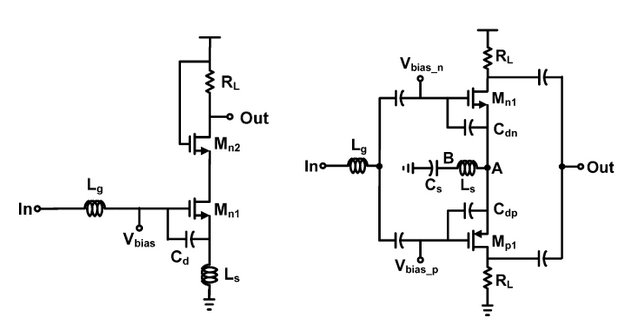
\includegraphics[width=0.5\textwidth]{figures/LNA.png}
    \caption{Cascade (left) and Current Reuse (right) structure ~\cite{lna}}
    \label{fig:lna}
\end{figure}

As the current reuse structure, the two common source amplifiers use the same drain to source current. The power consumption is minimized by using this kind of structure. Also, the gm parameter of this component is the $g_m$ of nFET plus the gm of pFET. In this way, the gain of this structure has been increased. The gain of the current reuse LNA is:

\begin{equation} 
  	\frac{g_{mtot}}{2R_s \omega_0 C_{gs}}Z_{load}
	\label{eq:lnagain}
\end{equation}

Here the $C_{gs}$ in ~\ref{eq:lnagain} is the total $C_{gs}$ of nFET and pFET. Also, the two transistors in the current reuse structure can be biased into subthreshold region to minimize the power consumption. The input matching should be matched to 50 $\Omega$. From the gates of the transistors, input impedance is:

\begin{equation} 
  	\frac{g_mL_s}{C_{gs}} + j[\omega (L_s+L_g) - \frac{1}{\omega C_{gs}}]
	\label{eq:inputimp}
\end{equation}

The real part in ~\ref{eq:inputimp} should be matched to 50 $\Omega$, and imaginary part should be matched to 0 $\Omega$. The input can be easily matched. The output, however, is difficult to be matched. The output impedance of this structure is:

\begin{equation} 
  	r_0 + j\frac{\omega(r_0g_{mtot}L_s+L_s-\omega^2L_sL_gC_{gs})}{1-(L_s+L_g)C_{gs}\omega^2}
\end{equation}

The imaginary part has the two same poles, also the pole is considered to be the central frequency. At the central frequency, the imaginary part goes to infinite, which makes it difficult to do the output matching. Because of this reason, cascade structure is used.

In cascade structure, the common source amplifier is the main amplifier. By applying the common gate, a good reverse isolation property is obtained. Fortunately, the input impedance of this structure is the same as the current reuse one (~\ref{eq:inputimp}). Thus, the input matching can be easily achieved. The output impedance of the cascade structure is (ignore channel length modulation):

\begin{equation} 
  	\frac{SLR_L}{SL+R_L-\omega^2LCR_L}
\end{equation}

At the central frequency, the output impedance equals to the load resistance. For matching the output, the load resistance is similar to the input impedance of next stage of the system, which is 500 $\Omega$. To analysis the gain parameters, the equation of cascade structure gain is derived: 

\begin{equation} 
  	\frac{R_L}{2\omega_0L_s}
\end{equation}

The load resistor and central frequency is fixed. To get a high gain LNA, the only free parameter can be adjusted is the source degenerated inductor. But, this inductor can affect the input matching. Therefore, the value of all of the components should be carefully selected. Cadence simulator is used to do the simulation of the proposed LNA. 

\subsection{Mixer}

A mixer takes two signals and produces an output that contains both the sum and the difference of the frequencies of the original signals. Mixers can be subclassed into active mixers and passive mixers. For our purposes, we need the mixer stage to exhibit some gain to meet design criteria so passive mixers were never considered. 

Internally, active mixers split down into single balanced and double balanced mixers. Double-balanced mixers can provide better input linearity, relatively low noise, and completely isolate the LO to RF ports resulting in very little feedthrough when compared to single balanced mixers. The cons are that the circuit requires large off-chip baluns/transformers to split the signal outputs if the other components do not do it already. 

\subsubsection{Design Procedure}
The typical mixer implementation is a standard Gilbert cell, which is a stock double-balanced mixer. The Gilbert cell original design doesn't have low noise, consumes relatively high power (for MedRadio), and needs to operate from a much larger supply voltage (must be capable of activating all transistors across ground). We employed the modified Gilbert cell from [AUTHOR] [REFERENCE]. It is pictured in Figure~\ref{fig:mixer}. 

\begin{figure}[h]
   \centering
    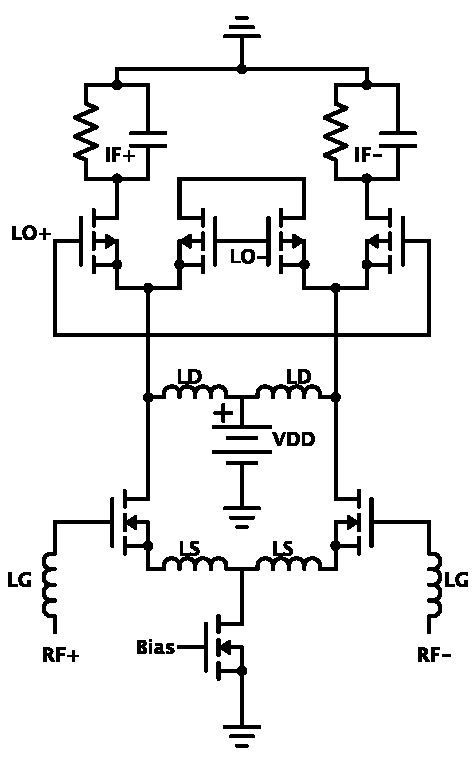
\includegraphics[width=0.40\textwidth]{figures/Mixer.pdf}
    \caption{
        Circuit schematic of the modified Gilbert cell used in our mixer. The top row of pMOS transistors are the switching pairs. The middle row of nMOS transistors are the transconductors with current being driven by the current sink at the bottom.
    }
    \label{fig:mixer}
\end{figure}

The advantages of this circuit is that the biasing of the switching pairs and the transconductors are now totally separated, allowing it to operate at a lower supply voltage without weakening circuit operation. The transconductors have control over the gain portion of the circuit and need to have careful current control through them, hence a current sink is connected to the source of the MOSFETs. For the switching pairs, the pMOS are biased to be barely on; mostly off.  The VCO signal will come into the switching pairs and quickly switch it into saturation and then back out again. It is to our disadvantage if the switching pairs enter the triode region since that will reduce the linearity and cause the gain to compress faster. 

The source and gate inductors connected to the transconductors are selected for input matching and to resonate the circuit. The drain inductor is sized to resonate with the VCO's parasitic source capacitance. Accordingly, the input impedance is given by:

\begin{equation} 
  	Z_{in}(j\omega) = \frac{g_{m}}{C_{gs}}L_{source}+j(\omega[L_{source}+L_{gate}]-\frac{1}{\omega C_{gs}})
	\label{eq:mixerZin}
\end{equation}

The resonance frequency is given by:

\begin{equation}
\omega = \frac{1}{\sqrt{C_{gs}(L_{source}+L_{gate})}}
\end{equation}

The source inductor is selected to match to an input resistance:

\begin{equation}
L_{source} = \frac{R_{input}}{\frac{g_{m}}{C_{gs}}}
\end{equation}

While the gate inductor is selected to achieve resonance at the input frequency to the transconductors:

\begin{equation}
L_{gate}=\frac{1-\omega^{2}L_{source}C_{gs}}{\omega^{2}C_{gs}}
\end{equation}

With these equations, the values of the gate and drain inductors can be properly chosen.
The conversion gain of the double balanced mixer is given typically by:

\begin{equation}
C.G. = \frac{2}{\pi}g_{m}Z_{out}
\end{equation}

Because of the input matching the transconductance term is modified and the final equation becomes:
\begin{equation}
C.G. = \frac{1}{\pi}\frac{g_{m}Z_{out}}{\sqrt{(1-\omega^{2}L_{source}C_{gs})^{2}+(\omega L_{source}g_{m})^{2}}}
\end{equation}

As a starting point, we made an assumption for the value of $C_{gs}$ using estimates culled from the IBM7RF library for the nMOS transistors and also assumed the output impedance was a single load resistor matched to 50 $\Omega$. Using that, we were able to make substitutions into the C.G. equation and solved for the desired value of the transconductance. After that, the input inductors were sized using the previous equations and assuming a center frequency of 403.5 MHz. Our initial design estimate assumed the current to start at 1 mA and we were able to get the sizing ratio using the below:

\begin{equation}
\frac{W}{L} = \frac{g_{m}^2}{2K_{n}I}
\end{equation}

Finally, the drain inductor values were obtained assuming simple resonance:

\begin{equation}
L_{drain} = \frac{1}{\sqrt{\omega^{2}_{VCO}C_{gs}}}
\end{equation}

At this point, the circuit was fully sized and allowed us to begin iterating the design to achieve the desired results.
The parameters that affected our results the most are as follows:

\begin{itemize}
	\item Width. This affected virtually every figure of merit (noise, gain, linearity), so it had to be tuned with great care. Accordingly, we wanted to keep the width below the millimeter scale at all costs.
	\item Switching DC bias and VCO swing. The DC bias of the was selected at a point where the VCO would have to swing as little as possible to switch the transistor from off to saturation (in order to reduce VCO power consumption). This primarily affected the gain and linearity of the circuit.
	\item Transistor fingers. The more fingers available lowered the parasitics of the transconductor stages. Increasing the fingers led to improved noise figure and linearity.
	\item Input impedance. The value of the input impedance had a large effect on our noise figure; we opted to increase the value we input matched to in order to reduce our overall noise.
	\item Output impedance. We needed to increase the gain without increasing the current. The only way to do that was to increase the size of the load resistor.
	\item Inductor values. The inductor values needed to be swept to compensate for tradeoffs between linearity and gain. The source inductor was kept relatively constant but the gate and drain inductors were tweaked often in an effort to improve the linearity of the mixer.
\end{itemize}

These are a small subset of the variables used when 

\subsection{Voltage Controlled Oscillator}
As shown in Figure ~\ref{fig:vco}, the proposed single-ended VCO uses a pair of complementary np-MOSFETs so that the dc current can be reused and a low power VCO can be realized ~\cite{vco}. The LC tank will determine the oscillation frequency by:

\begin{equation}
f_0 = \frac{1}{2\pi\sqrt{L_2C_V}}
\end{equation}

Note that, $C_V$ includes varactors, gate-source and drain-source capacitors of np-MOSFETs. The varactors are used to tune the VCO oscillation frequency. And on the other hand, the transistors are configured to provide a negative resistance to compensate the tank loss. 

\begin{figure}[h]
   \centering
    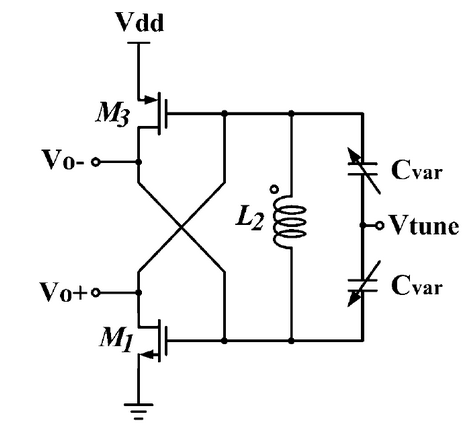
\includegraphics[width=0.50\textwidth]{figures/VCO.png}
    \caption{Schematic of the proposed VCO}
    \label{fig:vco}
\end{figure}


The nMOS has the dimension of $\frac{L}{W}=\frac{0.18}{30}$ and the pMOS has the dimension of $\frac{L}{W}=\frac{0.18}{200}$, both in micro. The values for inductor and varactors are optimized to center the oscillation frequency at 400 MHz. Note that, for better estimation of the VCO performance, all the capacitors, inductors and resistors are used as non-ideal components in the Cadence simulation. 

